% =====================================================================
% Part 1: Introduction through the Hough detector (sections 1–6)
% Included by explanation.tex.
% =====================================================================

\section{Introduction and Motivation}
\label{sec:intro}

Lane keeping is, by a comfortable margin, the most widely deployed
function in modern advanced driver-assistance systems (ADAS). Every
mass-market car with ``lane-keep assist'' or ``lane-centering'' on its
spec sheet contains -- somewhere behind a windshield-mounted camera --
some version of the pipeline this document explains. The economics are
unromantic but compelling: a \$20 image sensor, a \$2 microcontroller,
and a few thousand lines of code can subtract the most common cause of
single-vehicle highway crashes (drift out of lane due to inattention or
drowsiness). For the same reason, lane detection has become a
near-universal entry point into autonomy: it is geometrically simple,
visually intuitive, and tractable on a CPU. It is therefore an ideal
classroom problem -- a tiny slice of self-driving that nevertheless
exercises camera calibration, image processing, edge detection, line
fitting, polynomial regression, vehicle dynamics, and feedback control.

\paragraph{The perception--planning--control split.}
Autonomous-driving stacks are almost always organised into three
layers, executed once per frame in a fixed pipeline:
\begin{enumerate}[leftmargin=2em,itemsep=2pt]
  \item \textbf{Perception} -- read the camera (and, in real cars,
        radar, LiDAR, IMU), and produce a structured description of the
        world: ``the left lane boundary is the curve $x = a y^2 + b y + c$''.
  \item \textbf{Planning} -- from that description, decide where the
        car should be in the next few hundred milliseconds: ``stay
        centred between the boundaries with a small look-ahead''.
  \item \textbf{Control} -- compute the steering and throttle commands
        that drive the vehicle toward that target, given the vehicle's
        current dynamic state.
\end{enumerate}
In this project the same split is visible: \texttt{lane\_methods.py}
implements perception, the lane-centre target is computed implicitly as
``the midpoint of the two boundary curves'', and \texttt{controller.py}
implements two control laws (PID and Stanley). The simulator -- the
\texttt{camera.py} renderer, the \texttt{track.py} spline and the
\texttt{vehicle.py} bicycle model -- replaces the physical world.

\paragraph{Why classical CV rather than deep learning?}
A naive reading of the recent literature might suggest the problem is
``solved'' by learning. State-of-the-art lane detectors -- LaneNet,
SCNN, PolyLaneNet, Ultra-Fast-Lane-Detection -- learn an end-to-end
map from pixels to lane parameters and dominate every public benchmark
(TuSimple, CULane, LLAMAS). Why then would anyone deploy a
hand-written Canny + Hough pipeline in 2026?
\begin{itemize}[leftmargin=1.4em,itemsep=2pt]
  \item \textbf{Interpretability.} Every step of the classical pipeline
        has a closed-form mathematical definition. If the car
        misbehaves, the failure can be traced to a specific stage: the
        ROI was wrong, the threshold was too high, the Hough binning
        was too coarse. With a black-box CNN this kind of forensic
        analysis is far harder.
  \item \textbf{Compute footprint.} The full pipeline in this project
        runs at $>1000$ FPS on a single CPU thread; a learned
        segmenter typically needs a GPU or NPU. For low-end ADAS
        modules without an accelerator, classical CV is the only
        option.
  \item \textbf{No training data, no labelling, no domain shift.}
        A classical detector contains no learned weights, so there is
        no train/test distribution mismatch. Its assumptions are
        visible (``edges of constant gradient form lines''), so we can
        predict \emph{a priori} where it will fail.
  \item \textbf{Educational clarity.} For a course project, every line
        of \texttt{HoughDetector.detect} is a piece of mathematics we
        can derive. Every line of a UNet is opaque.
\end{itemize}
The trade-off is equally clear: classical detectors assume a clean,
high-contrast world. They struggle with shadows, weathered paint,
crowded roads, and -- as we will see in detail -- with curves. The
question this project answers is therefore very specific: given that
the textbook Hough lane detector clearly fails on curves, how much of
that gap can be closed by a slightly less classical method that still
avoids deep learning? The proposed answer -- a bird's-eye
sliding-window quadratic fit -- reduces RMS lateral error by $34\%$ on
average across five tracks, while remaining interpretable and
real-time.

\paragraph{Roadmap of this document.}
This document is the long-form, pedagogical companion to the project.
The short report (\texttt{presentation/report.tex}) gives the
experimental punch line in three pages; this document gives every
derivation, every worked example, and every line of code behind the
punch line.
\begin{itemize}[leftmargin=1.4em,itemsep=2pt]
  \item Section~\ref{sec:prelim} covers the mathematical preliminaries:
        images as functions, colour spaces, convolution, Gaussian
        smoothing, the Sobel operator, and the four steps of the Canny
        edge detector. If you have not seen these before, this is
        where to spend the most time.
  \item Section~\ref{sec:sim} dissects the simulator: the
        Catmull--Rom spline that defines each track, the discrete
        curvature formula, the bicycle kinematic model, and the
        pinhole camera that produces the first-person image the
        detectors see.
  \item Section~\ref{sec:sub} formalises the lane-detection sub-problem:
        what the detectors are asked to compute, and what ground truth
        is available for evaluation.
  \item Section~\ref{sec:centroid} works through the first detector --
        the centroid baseline -- and explains, with image moments, why
        it cannot possibly succeed.
  \item Section~\ref{sec:hough} works through the second detector --
        the Hough-line pipeline -- in full mathematical detail,
        including the polar parameterisation of a line, the
        probabilistic Hough variant used by OpenCV, slope
        classification, length-weighted averaging, and temporal
        exponential smoothing.
\end{itemize}
The second half of the document (Part~2) picks up with the
inverse-perspective mapping and the proposed polynomial-fit detector,
then continues into vehicle control and the experimental evaluation.

% =====================================================================
\section{Mathematical Preliminaries}
\label{sec:prelim}

Before we can speak meaningfully about ``detecting lanes'' we need to
agree on what an image is, and on the handful of operations we will
perform on it. This section is deliberately slow: a third-year CS
student who has never taken a CV class should be able to follow every
formula and reproduce every numerical example by hand.

\subsection{An image is a function}

\begin{definition}[Discrete image]
A grayscale image of width $W$ and height $H$ is a function
\[
I : \{0,\ldots,W-1\}\times\{0,\ldots,H-1\}\to\{0,\ldots,255\},
\]
mapping integer pixel coordinates $(u,v)$ to an 8-bit intensity. A
colour image has the same domain but a three-component codomain,
$I:(u,v)\mapsto(R,G,B)\in\{0,\ldots,255\}^3$.
\end{definition}

Two conventions must be stated explicitly because they trip up almost
every newcomer:
\begin{enumerate}[leftmargin=2em,itemsep=2pt]
  \item The origin is at the \emph{top-left} of the image. The first
        axis $u$ increases to the right; the second axis $v$ increases
        downward. This is opposite to the convention you learned in
        calculus class, where $y$ usually points up.
  \item In our simulator the world coordinate $(X,Y)$ uses the same
        screen-down convention as the image (because everything is
        drawn into a Pygame window whose origin is also top-left). Be
        careful not to confuse image pixels and world pixels: the
        camera's $640\times480$ frame is one coordinate system; the
        $1400\times800$ Pygame window is another.
\end{enumerate}
The camera in this project produces images of size $W=640$, $H=480$
(set in \texttt{config.py}: \texttt{CAMERA\_IMG\_W=640},
\texttt{CAMERA\_IMG\_H=480}). A single frame is a NumPy array of shape
\texttt{(480, 640, 3)} with \texttt{dtype=uint8}.

\subsection{RGB to grayscale}

The first thing every classical detector in this project does is throw
away colour: it converts the RGB image to a single-channel grayscale
image. The standard conversion follows ITU-R Recommendation BT.601
(``Rec.~601''), originally designed so that the luminance channel of
analogue colour television matches what a human eye perceives as
brightness:
\begin{equation}
Y = 0.299\,R + 0.587\,G + 0.114\,B.
\label{eq:gray}
\end{equation}
The coefficients are not arbitrary: the human eye is much more
sensitive to green than to red, and least sensitive to blue. A simple
unweighted average $(R+G+B)/3$ would make red and green grass look
almost identical even though they are visually obviously different.

\begin{example}[Grayscale of a road pixel]
Our simulator paints the road in $\text{RGB}=(64,68,74)$ (see
\texttt{config.py:ROAD\_SURFACE}). Applying \eqref{eq:gray}:
\[
Y = 0.299\cdot 64 + 0.587\cdot 68 + 0.114\cdot 74
  \approx 19.14 + 39.92 + 8.44 \approx 67.5.
\]
So the road has roughly intensity 68 on a $[0,255]$ scale -- a fairly
dark grey, but well above black. Compare to grass
$\text{RGB}=(34,52,30)$: $Y\approx 10.2+30.5+3.4 = 44.1$. The road is
about $50\%$ brighter than the grass; that contrast is what lets the
Canny edge detector discover the road boundary.
\end{example}

In OpenCV the call is \texttt{cv2.cvtColor(img, cv2.COLOR\_RGB2GRAY)}
and it is the very first line of every \texttt{detect()} method in
this project (e.g.\ \texttt{lane\_methods.py:HoughDetector.detect},
line~203).

\subsection{The HSV colour space}

Sometimes we want to threshold by colour rather than brightness -- for
example, to find the yellow centre dashes
(\texttt{LANE\_DASH\_COLOR}\,=\,(200,200,80)) regardless of how
brightly lit they are. RGB is awkward for this because ``yellow'' is
a curve in 3-space rather than an axis; HSV separates the perceptual
axes:
\begin{itemize}[leftmargin=1.4em,itemsep=2pt]
  \item \textbf{Hue} $H\in[0,360^\circ)$: which colour. Red $\approx 0$,
        yellow $\approx 60$, green $\approx 120$, cyan $\approx 180$,
        blue $\approx 240$, magenta $\approx 300$. (OpenCV stores $H$
        scaled to $[0,180)$ so it fits in a \texttt{uint8}.)
  \item \textbf{Saturation} $S\in[0,1]$: how colourful. $S=0$ is pure
        grey; $S=1$ is fully saturated.
  \item \textbf{Value} $V\in[0,1]$: how bright. $V=0$ is black; $V=1$
        is the brightest version of the hue.
\end{itemize}
The conversion is piecewise. Given $R,G,B\in[0,1]$, let
$M=\max(R,G,B)$, $m=\min(R,G,B)$ and $C=M-m$. Then $V=M$, $S=C/M$ (if
$M>0$, else $0$), and
\[
H = 60^\circ\cdot
\begin{cases}
   \dfrac{G-B}{C}\bmod 6, & M=R,\\[4pt]
   \dfrac{B-R}{C} + 2,    & M=G,\\[4pt]
   \dfrac{R-G}{C} + 4,    & M=B.
\end{cases}
\]

\begin{example}[HSV of the road pixel]
Take the road colour $(R,G,B)=(64,68,74)$. Normalise to $[0,1]$:
$(0.251,0.267,0.290)$. Then $M=0.290$ (the blue channel), $m=0.251$,
$C=0.039$.
\begin{align*}
V &= 0.290 \;\Rightarrow\; V\cdot 255 \approx 74,\\
S &= C/M = 0.039/0.290 \approx 0.135 \;\Rightarrow\; S\cdot 255 \approx 34,\\
H &= 60^\circ\!\left(\tfrac{R-G}{C}+4\right)
   = 60^\circ\!\left(\tfrac{-0.016}{0.039}+4\right)
   \approx 60^\circ\cdot 3.59 \approx 215^\circ.
\end{align*}
So the road sits at hue $\approx 215^\circ$ (a slightly cool
blue-grey, which is correct -- the colour is barely off neutral), low
saturation $\approx 34/255$, and moderate value $\approx 74/255$. The
\texttt{CentroidDetector} uses precisely this signature to threshold
the road: \texttt{(s<40) \& (v>40) \& (v<110)} (line~122 of
\texttt{lane\_methods.py}). The chosen bounds bracket exactly the
$(S,V)$ values we just computed.
\end{example}

\subsection{2D convolution}

Everything we do to the image after grayscale conversion -- blurring,
edge detection, gradient estimation -- is a linear filter, and every
linear filter can be written as a convolution between the image $I$
and a small kernel $K$.

\begin{definition}[2D discrete convolution]
Given image $I$ and kernel $K$ of size $(2k{+}1)\times(2k{+}1)$, the
convolution $(I*K):\mathbb{Z}^2\to\mathbb{R}$ is
\begin{equation}
(I*K)(u,v) = \sum_{i=-k}^{k}\sum_{j=-k}^{k}
            I(u-i,v-j)\,K(i,j).
\label{eq:conv}
\end{equation}
\end{definition}

The minus signs in \eqref{eq:conv} are not a typo: a true convolution
flips the kernel before sliding it. In practice many image-processing
libraries (OpenCV included) actually compute the \emph{correlation}
$(I\star K)(u,v) = \sum_{i,j} I(u+i,v+j)K(i,j)$ -- with no flip -- and
call it convolution. For symmetric kernels (Gaussian, mean,
Sobel-magnitude\footnote{Sobel $S_x$, $S_y$ are antisymmetric, but the
sign convention is folded into the definition; what matters is being
consistent.}) the two operations agree, so the pedantry rarely bites.

\begin{example}[A $3\times 3$ box blur]
Consider a tiny grayscale image and a $3\times 3$ averaging kernel:
\[
I = \begin{pmatrix}10 & 20 & 30 \\ 40 & 50 & 60 \\ 70 & 80 & 90\end{pmatrix},\quad
K = \frac{1}{9}\begin{pmatrix}1&1&1\\1&1&1\\1&1&1\end{pmatrix}.
\]
At the centre pixel $(1,1)$ the convolution is the mean of all nine
values, $(10+20+\cdots+90)/9 = 450/9 = 50$. So $(I*K)(1,1)=50$. At a
boundary pixel we have to decide how to handle the missing neighbours;
OpenCV by default replicates the edge value, but the convolution
formula is identical otherwise.
\end{example}

\subsection{The Gaussian kernel}

Random pixel noise (and noise added in our experiments via
\texttt{evaluate.py:\_add\_noise}) is the enemy of edge detection: a
single bright spike inside an otherwise smooth patch produces a strong
gradient that no edge actually exists. The standard remedy is to blur
the image with a Gaussian kernel before computing gradients:
\begin{equation}
G_\sigma(x,y) = \frac{1}{2\pi\sigma^2}\exp\!\left(-\frac{x^2+y^2}{2\sigma^2}\right).
\label{eq:gauss}
\end{equation}
The function is rotationally symmetric and integrates to $1$ over
$\mathbb{R}^2$; in discrete form we sample \eqref{eq:gauss} at integer
offsets, then renormalise so the sampled values sum exactly to $1$ (to
preserve average brightness).

\begin{example}[$5\times 5$ Gaussian with $\sigma=1$]
Sampling \eqref{eq:gauss} at $(x,y)\in\{-2,-1,0,1,2\}^2$ with
$\sigma=1$ gives the unnormalised values
\[
\tilde G=\begin{pmatrix}
0.0030 & 0.0133 & 0.0219 & 0.0133 & 0.0030\\
0.0133 & 0.0596 & 0.0983 & 0.0596 & 0.0133\\
0.0219 & 0.0983 & 0.1620 & 0.0983 & 0.0219\\
0.0133 & 0.0596 & 0.0983 & 0.0596 & 0.0133\\
0.0030 & 0.0133 & 0.0219 & 0.0133 & 0.0030
\end{pmatrix}.
\]
The entries sum to about $0.9989$, so renormalising hardly changes
them. A common integer approximation (used in many introductory
tutorials) is
\[
G = \frac{1}{273}\begin{pmatrix}
1 & 4 & 7 & 4 & 1\\
4 & 16 & 26 & 16 & 4\\
7 & 26 & 41 & 26 & 7\\
4 & 16 & 26 & 16 & 4\\
1 & 4 & 7 & 4 & 1
\end{pmatrix},
\]
whose centre value $41/273\approx 0.150$ is close to the exact
$0.162$. Our project calls
\texttt{cv2.GaussianBlur(gray, (5,5), 0)} (line~204 of
\texttt{lane\_methods.py}); passing $\sigma=0$ tells OpenCV to derive
$\sigma$ from the kernel size as
$\sigma = 0.3((k-1)/2-1)+0.8\approx 1.1$, which is essentially the
kernel we just built.
\end{example}

A larger $\sigma$ blurs more aggressively, removes finer noise, but
also smears out genuine edges. The $5\times 5$ kernel with
$\sigma\approx 1$ is a good default for $640\times 480$ images: it
attenuates pixel-scale noise without dissolving lane markings.

\subsection{Image gradients: the Sobel operator}

An edge is, intuitively, a place where the image brightness changes
rapidly. Mathematically: a place where the spatial derivative
$\nabla I$ has a large magnitude. To approximate $\nabla I$ on a
discrete grid we convolve with the Sobel kernels:
\begin{equation}
S_x = \begin{pmatrix}-1 & 0 & 1\\-2 & 0 & 2\\-1 & 0 & 1\end{pmatrix},\quad
S_y = \begin{pmatrix}-1 & -2 & -1\\ 0 & 0 & 0\\ 1 & 2 & 1\end{pmatrix}.
\label{eq:sobel}
\end{equation}
Each kernel is the discrete tensor product of a smoothing kernel
$(1,2,1)$ in one direction with a central-difference derivative
$(-1,0,1)$ in the other; you can think of $S_x$ as ``smooth vertically
then differentiate horizontally''. The output channels $G_x=I*S_x$ and
$G_y=I*S_y$ are the estimated partial derivatives; gradient magnitude
and direction follow:
\begin{equation}
|G| = \sqrt{G_x^2+G_y^2},\qquad
\alpha = \operatorname{atan2}(G_y,G_x).
\label{eq:grad}
\end{equation}
The \texttt{PolyFitDetector} uses $S_x$ explicitly to find
vertical-ish lane markings (line~406 of \texttt{lane\_methods.py}:
\texttt{cv2.Sobel(gray, cv2.CV\_32F, 1, 0, ksize=3)}). The Hough
detector does not call Sobel directly because the Canny edge detector
(below) does it internally.

\subsection{Canny edge detection}

\texttt{cv2.Canny} reduces a grayscale image to a binary edge map:
pixel $(u,v)$ is $255$ if Canny believes there is an edge there, and
$0$ otherwise. The Canny algorithm (Canny 1986) is composed of four
steps that are all worth understanding individually:
\begin{enumerate}[leftmargin=1.6em,itemsep=2pt]
  \item \textbf{Gaussian blur.} As described above, smooth the image
        to suppress single-pixel noise. Without this step the
        derivatives in step~2 would amplify every speckle.
  \item \textbf{Sobel gradients.} Compute $G_x,G_y$ and the gradient
        magnitude $|G|$ from \eqref{eq:grad}. The magnitude image
        already looks like an edge map -- but it is too thick (real
        edges are typically several pixels wide because the gradient
        is non-zero across the whole transition), and includes weak
        responses everywhere.
  \item \textbf{Non-maximum suppression.} For each pixel, check
        whether its gradient magnitude is larger than that of its two
        immediate neighbours along the gradient direction $\alpha$. If
        not, zero it out. This thins the edge map to single-pixel-wide
        ridges, which is what we need for line fitting.
  \item \textbf{Double-threshold hysteresis.} A high threshold $T_H$
        marks ``strong'' edges; a low threshold $T_L$ marks
        ``candidate'' edges. A candidate edge is retained iff it is
        connected (8-neighbourhood) to a strong edge. This hysteresis
        is what makes Canny robust: an edge that peaks weakly but is
        part of a long contour survives, while isolated weak edges
        (noise) are discarded.
\end{enumerate}
This project uses \texttt{cv2.Canny(blurred, 50, 150)} with
$T_L=50$, $T_H=150$ (\texttt{config.py:CANNY\_LOW=50},
\texttt{CANNY\_HIGH=150}). The classical heuristic is $T_H:T_L$
between $2{:}1$ and $3{:}1$; we use exactly $3{:}1$. These specific
numbers were tuned against the simulator's road colours: $50$ is just
above the noise floor of the rendered frame, and $150$ comfortably
excludes everything except the sharp lane-boundary edges.

\begin{intuition}
An edge is where the image brightness changes fast in some direction.
Canny finds those places, thins the response so each edge is exactly
one pixel wide, and then keeps only the ones long enough (via
hysteresis) to be a real contour rather than a stray noise spike.
Everything else in the lane-detection pipeline operates on this
thinned binary picture.
\end{intuition}

% =====================================================================
\section{The Driving Simulator}
\label{sec:sim}

The simulator is small but it is doing a surprising amount of work:
generating a smooth closed-loop track, computing its curvature,
simulating a kinematic bicycle vehicle, and rendering the world
through a virtual pinhole camera. We treat each piece in turn.

\subsection{Track geometry: the Catmull--Rom spline}

A track in \texttt{config.py} is a list of $n$ waypoints
$\mathbf{p}_0,\mathbf{p}_1,\ldots,\mathbf{p}_{n-1}\in\mathbb{R}^2$
(e.g.\ 12 for the oval, 21 for Red Bull Ring). Connecting them with
straight line segments would give a polygon, not a track -- the
resulting heading changes would be discontinuous, the steering would
saturate at every waypoint, and the simulation would look terrible. We
need a smooth curve that passes through every waypoint.

\begin{definition}[Catmull--Rom spline]
Given four control points $\mathbf{p}_0,\mathbf{p}_1,\mathbf{p}_2,\mathbf{p}_3$,
the Catmull--Rom spline segment between $\mathbf{p}_1$ and
$\mathbf{p}_2$ is
\begin{equation}
\mathbf{q}(t)=\tfrac{1}{2}\Big[
  (2\mathbf{p}_1)
  + (-\mathbf{p}_0+\mathbf{p}_2)\,t
  + (2\mathbf{p}_0-5\mathbf{p}_1+4\mathbf{p}_2-\mathbf{p}_3)\,t^2
  + (-\mathbf{p}_0+3\mathbf{p}_1-3\mathbf{p}_2+\mathbf{p}_3)\,t^3
\Big],
\label{eq:catmull}
\end{equation}
for $t\in[0,1]$. The spline passes through $\mathbf{p}_1$ at $t=0$ and
$\mathbf{p}_2$ at $t=1$, while $\mathbf{p}_0$ and $\mathbf{p}_3$ control
the tangents at the endpoints.
\end{definition}

To check the interpolation property, substitute $t=0$ into
\eqref{eq:catmull}: the $t^1,t^2,t^3$ terms vanish, leaving
$\mathbf{q}(0)=\tfrac{1}{2}\cdot 2\mathbf{p}_1 = \mathbf{p}_1$.
Likewise $t=1$ gives $\mathbf{q}(1)=\mathbf{p}_2$. Differentiating,
\[
\mathbf{q}'(0)=\tfrac{1}{2}(\mathbf{p}_2-\mathbf{p}_0),\qquad
\mathbf{q}'(1)=\tfrac{1}{2}(\mathbf{p}_3-\mathbf{p}_1),
\]
so the tangent at $\mathbf{p}_1$ is parallel to the chord
$\mathbf{p}_2-\mathbf{p}_0$ -- the segment ``aims through'' the next
waypoint. The same tangent value is shared by the adjacent segment, so
the assembled curve is $C^1$-continuous (no kinks in heading) through
every waypoint. That is exactly what a drivable track needs.

In code (\texttt{track.py:Track.\_interpolate}, lines~31--52), the
spline is sampled at \texttt{TRACK\_SAMPLES\_PER\_SEGMENT~=~60} values
of $t\in[0,1)$ per segment, looping the index modulo $n$ so the track
closes back to its first waypoint. For the 12-waypoint oval this gives
$12\times 60 = 720$ centreline samples, dense enough that
finite-difference tangents and curvatures are well-behaved.

\subsection{Curvature of a parametric curve}

Once we have the centreline as a parametric curve $\mathbf{c}(s)=(x(s),y(s))$,
we often want its curvature -- how sharply it is bending. Two reasons:
(i)~the adaptive-speed controller slows the car before curves, so it
needs to know which sections are sharp; (ii)~the Hough detector's
main failure mode is that it cannot represent curvature, so
understanding how curved each track is tells us where to expect Hough
to break.

\begin{definition}[Curvature of a 2D parametric curve]
For a curve $(x(s),y(s))$ with finite first and second derivatives,
the (signed) curvature is
\begin{equation}
\kappa(s)=\frac{x'(s)\,y''(s)-y'(s)\,x''(s)}{\bigl(x'(s)^2+y'(s)^2\bigr)^{3/2}}.
\label{eq:kappa}
\end{equation}
\end{definition}

The simulator uses the unsigned version $|\kappa|$ (it only cares
about ``how curvy'', not ``which way''), implemented in
\texttt{track.py:Track.\_compute\_curvature} on lines~68--103 via
central differences:
\[
\dot x_i\approx \tfrac{x_{i+1}-x_{i-1}}{2},\qquad
\ddot x_i\approx x_{i+1}-2x_i+x_{i-1},
\]
and similarly for $y$. The grid spacing is absorbed into the
$(\cdot)^{3/2}$ factor in the denominator, which is why the formula in
code has no explicit $\Delta s$.

\paragraph{Units.}
If $(x,y)$ are in pixels and the parameter $s$ is also in pixels, then
$x'$ is dimensionless, $x''$ has units of $1/\text{px}$, and the
numerator of \eqref{eq:kappa} has units of $1/\text{px}$. The
denominator $(x'^2+y'^2)^{3/2}$ is dimensionless. So $\kappa$ has
units of $1/\text{px}$, which equals $1/R$ for a circle of radius $R$
-- exactly what curvature should be.

After computing $\kappa$ point-by-point, the simulator smooths the
result with a 15-point rolling average (lines~100--102) to suppress
spline-sampling jitter; only then is it used by the
\texttt{SpeedController}.

\subsection{Bicycle kinematic model}

The vehicle's state at time $t$ is the triple $(x(t),y(t),\theta(t))$
-- position and heading -- plus a scalar forward speed $v$ and a
steering angle $\delta$. We need a differential equation that says how
$(x,y,\theta)$ evolves as a function of $v$ and $\delta$.

The \emph{bicycle kinematic model} makes one simplifying assumption:
the left and right wheels of each axle are collapsed into a single
wheel on the centreline, so the car becomes a bicycle. Two further
assumptions follow from this:
\begin{enumerate}[leftmargin=2em,itemsep=2pt]
  \item \textbf{No side slip.} Each wheel's velocity vector is aligned
        with the direction the wheel is pointing. The rear wheel
        points along the body's heading $\theta$; the front wheel
        points along $\theta+\delta$.
  \item \textbf{Rear-axle reference.} We track the position of the
        rear axle. This is convenient because the rear wheel's
        velocity equals the body's velocity in the body frame.
\end{enumerate}
Under these assumptions the velocity of the rear axle is just
$(v\cos\theta, v\sin\theta)$. To find how fast $\theta$ changes,
observe that during a small time $dt$ the rear and front axles each
move forward by $v\,dt$, but the front axle moves along heading
$\theta+\delta$ while the rear moves along $\theta$. The front axle
must therefore swing around the rear by an angle $d\theta$ such that
the front-axle displacement perpendicular to the body, $v\,dt\sin\delta$,
equals $L\,d\theta$ (where $L$ is the wheelbase). Hence
$\dot\theta = (v\sin\delta)/L\cdot(1/\cos\delta) = (v/L)\tan\delta$
once you keep the projection along the body axis consistent.

The full system is therefore
\begin{equation}
\dot x = v\cos\theta,\quad
\dot y = v\sin\theta,\quad
\dot\theta = \frac{v}{L}\tan\delta.
\label{eq:bicycle}
\end{equation}

In code (\texttt{vehicle.py:Vehicle.update}, lines~19--31), this is
integrated by forward Euler: $x\leftarrow x + v\cos\theta\,\Delta t$,
$y\leftarrow y + v\sin\theta\,\Delta t$,
$\theta\leftarrow\theta + (v/L)\tan\delta\,\Delta t$. The steering
angle is first clamped to $\pm 40^\circ$ (\texttt{config.py:MAX\_STEERING\_ANGLE}).

\begin{example}[Instantaneous turn radius]
With $L=25$\,px, $\delta=20^\circ$ and $v=100$\,px/s, the bicycle's
instantaneous turn radius is
\[
R = \frac{L}{\tan\delta} = \frac{25}{\tan 20^\circ}\approx \frac{25}{0.364}\approx 68.7\text{ px},
\]
and the angular velocity is
\[
\dot\theta = \frac{v}{R} = \frac{100}{68.7}\approx 1.46\text{ rad/s},
\]
or about $83^\circ/$s -- the car would rotate $360^\circ$ in roughly
$4.3$\,s. Equivalently, $\dot\theta = (v/L)\tan\delta = (100/25)\cdot
0.364 = 1.46$\,rad/s, matching~\eqref{eq:bicycle}.
\end{example}

\subsection{The pinhole camera}

The camera in \texttt{camera.py} takes world points $(X,Y)$ -- on the
ground plane in front of the vehicle -- and produces image pixel
coordinates $(u,v)$. It is the most important piece of geometry in the
whole project, because every detector is fed the output of this
projection.

\subsubsection{Focal length from field of view}

A pinhole camera with image width $W$ and horizontal field of view
$\text{FoV}$ satisfies
\begin{equation}
\tan(\text{FoV}/2) = \frac{W/2}{f}\quad\Longleftrightarrow\quad
f = \frac{W/2}{\tan(\text{FoV}/2)}.
\label{eq:focal}
\end{equation}
With $W=640$ and $\text{FoV}=70^\circ$ (config),
\[
f = \frac{320}{\tan(35^\circ)}\approx\frac{320}{0.7002}\approx 457.0\text{ px}.
\]
This is the value computed on line~14 of \texttt{camera.py}:
\texttt{self.focal = (self.w / 2) / math.tan(fov\_rad / 2)}.

\subsubsection{Camera frame and pitch rotation}

The camera is mounted at height $h=50$\,px above the ground, pitched
down by $\varphi=18^\circ$. Define a vehicle-local frame whose origin
is on the ground directly beneath the camera, $+Z$ pointing forward
along the vehicle's heading, $+X$ pointing right, $+Y$ pointing down.
A ground point in front of the car has coordinates
$(X_{\text{lat}}, h, Z_{\text{fwd}})$ -- ``$h$'' because the ground is
$h$ pixels below the camera, which is the $+Y$ direction.

The camera frame after pitch is obtained by rotating around the $X$
axis by $\varphi$:
\begin{equation}
\begin{pmatrix}X_c\\Y_c\\Z_c\end{pmatrix} =
\begin{pmatrix}1 & 0 & 0\\ 0 & \cos\varphi & -\sin\varphi\\ 0 & \sin\varphi & \cos\varphi\end{pmatrix}
\begin{pmatrix}X_{\text{lat}}\\ h\\ Z_{\text{fwd}}\end{pmatrix}.
\label{eq:rot}
\end{equation}
Carrying out the multiplication explicitly,
\begin{equation}
\begin{aligned}
X_c &= X_{\text{lat}},\\
Y_c &= h\cos\varphi - Z_{\text{fwd}}\sin\varphi,\\
Z_c &= h\sin\varphi + Z_{\text{fwd}}\cos\varphi.
\end{aligned}
\label{eq:cam}
\end{equation}
These three lines are exactly lines~58--60 of \texttt{camera.py}.
Finally the perspective division gives image coordinates:
\begin{equation}
u = f\,\frac{X_c}{Z_c} + c_x,\quad
v = f\,\frac{Y_c}{Z_c} + c_y,
\label{eq:proj}
\end{equation}
where $(c_x,c_y)=(W/2,H/2)=(320,240)$ is the principal point. A point
is visible iff $Z_c>2$ (just in front of the camera; see line~63 of
\texttt{camera.py}).

\begin{example}[Projecting a ground point]
Take a point 200\,px directly ahead of the camera on the ground:
$X_{\text{lat}}=0$, $h=50$, $Z_{\text{fwd}}=200$. With
$\varphi=18^\circ$, $\cos\varphi\approx 0.951$,
$\sin\varphi\approx 0.309$:
\begin{align*}
X_c &= 0,\\
Y_c &= 50\cdot 0.951 - 200\cdot 0.309\approx 47.55 - 61.80 \approx -14.25,\\
Z_c &= 50\cdot 0.309 + 200\cdot 0.951 \approx 15.45 + 190.20 \approx 205.65.
\end{align*}
With $f\approx 457$,
\[
u = 457\cdot 0/205.65 + 320 = 320,\quad
v = 457\cdot(-14.25)/205.65 + 240 \approx -31.66+240 = 208.3.
\]
So this point projects to roughly $(320,208)$ -- horizontally centred
(it was straight ahead) and just above the image vertical centre 240,
which makes sense: with the camera pitched down, a point on the
horizon would lie below 240, while a point only 200\,px ahead is
nearer than the horizon and projects higher.
\end{example}

\subsubsection{The full FPV render}

\texttt{FPVCamera.render} (lines~79--141 of \texttt{camera.py}) puts
the above together for an entire frame:
\begin{enumerate}[leftmargin=1.8em,itemsep=2pt]
  \item Copy a pre-computed vertical sky gradient (lines~24--32).
  \item Compute the horizon row analytically: as $Z_{\text{fwd}}\to\infty$,
        equation~\eqref{eq:cam} gives $Y_c\to-Z_{\text{fwd}}\sin\varphi$
        and $Z_c\to Z_{\text{fwd}}\cos\varphi$, so
        $v_{\text{horizon}} = f\cdot(-\sin\varphi/\cos\varphi)+c_y
        = -f\tan\varphi + c_y$. Fill everything below that with grass.
  \item Ask the track for the left, right and centre boundary points
        within \texttt{CAMERA\_LOOK\_AHEAD~=~350}\,px of the vehicle
        (\texttt{Track.get\_road\_ahead}).
  \item Project those points through \eqref{eq:cam} and \eqref{eq:proj},
        drop the ones behind the camera, fill the polygon between left
        and right boundaries with the road colour
        \texttt{ROAD\_SURFACE = (64, 68, 74)}.
  \item Draw the solid white boundary lines and the dashed yellow
        centre line on top.
\end{enumerate}
The result is a $640\times 480$ RGB image -- the same shape and
content as if a real camera were filming a real road -- which is then
handed off to the lane detector. There is no real-world data anywhere
in the pipeline; the simulator \emph{is} the world.

\begin{intuition}
You can think of the camera as the inverse of the inverse-perspective
(IPM) warp we will meet in Section~\ref{sec:polyfit}. The camera takes
world points and projects them onto the image plane; the IPM takes
image pixels and projects them back onto the ground plane. The polyfit
detector explicitly inverts what the camera does.
\end{intuition}

% =====================================================================
\section{The Lane-Detection Sub-problem}
\label{sec:sub}

We have now described the world the detectors live in. What exactly
are they asked to do?

\subsection{Inputs and outputs}

Every lane detector in this project implements the same interface
(\texttt{lane\_methods.py:LaneDetectorBase}, line~81). It takes a
single input -- the current camera frame as an RGB NumPy array of
shape $(H,W,3)=(480,640,3)$ -- and returns a \texttt{Detection} object
with the following fields:
\begin{itemize}[leftmargin=1.4em,itemsep=2pt]
  \item \texttt{center\_offset}: signed horizontal offset (in camera
        pixels) of the detected lane centre from the image centre.
        Positive means the lane centre is to the right of the camera,
        so the car must steer right to centre itself.
  \item \texttt{lookahead\_offset}: the same quantity but evaluated
        further up the image (i.e.\ further ahead in world terms).
        Equal to \texttt{center\_offset} for line-based detectors;
        meaningfully different for the polyfit detector on curves.
  \item \texttt{confidence}: a scalar in $[0,1]$. The Hough detector
        returns $1$ if both boundaries were found, $0.5$ if only one,
        and $0$ if none.
  \item \texttt{pred\_mask}: a binary mask of the predicted lane
        polygon, used by the evaluator to compute
        intersection-over-union against the ground-truth road mask.
  \item \texttt{annotated}: an annotated copy of the input image (for
        the UI; not used by the controller).
\end{itemize}

\subsection{Ground truth available in the simulator}

Because the world is synthetic, we have access to two kinds of ground
truth that no real camera could ever provide:
\begin{enumerate}[leftmargin=2em,itemsep=2pt]
  \item \textbf{Signed lateral error.}
        \texttt{Track.get\_nearest\_index} (lines~154--164 of
        \texttt{track.py}) returns, for the vehicle's current
        $(x,y)$, the nearest centreline index and the signed
        perpendicular distance to the centreline. This is the true
        lateral error $e_\perp$ -- what every detector is trying to
        estimate.
  \item \textbf{Ground-truth lane polygon.} The function
        \texttt{evaluate.py:\_gt\_lane\_mask} (lines~68--84)
        re-projects the simulator's true road boundary polygon
        through the same pinhole camera used to render the input
        image, producing a $H\times W$ binary mask of where the road
        really is in the camera frame. The Lane-IoU metric is then
        $\text{IoU} = |\text{pred}\cap\text{gt}|/|\text{pred}\cup\text{gt}|$
        -- a single scalar in $[0,1]$ that summarises both the
        position and the shape of the predicted lane.
\end{enumerate}
Because all three detectors return a \texttt{pred\_mask} of the same
shape, they can be compared on the same IoU scale even though they
use very different internal representations.

\subsection{Preview of the three detectors}

Three detectors are implemented, in increasing order of sophistication:
\begin{itemize}[leftmargin=1.4em,itemsep=2pt]
  \item \textbf{Centroid} (Section~\ref{sec:centroid}). HSV-threshold
        the road, take the centroid of the resulting blob.
        Deliberately simple; serves as a lower bound.
  \item \textbf{Hough} (Section~\ref{sec:hough}). The textbook Canny
        + Hough pipeline. Fits a single straight line per lane
        boundary. Works on straights, struggles on curves.
  \item \textbf{Polyfit} (Section~\ref{sec:polyfit}, in Part~2).
        Inverse-perspective warp followed by a sliding-window
        quadratic fit. Can model curves explicitly.
\end{itemize}

% =====================================================================
\section{Detector 1 -- The Centroid Baseline}
\label{sec:centroid}

The \texttt{CentroidDetector} (lines~95--171 of
\texttt{lane\_methods.py}) is the simplest possible thing one could
try. It is included specifically so that we have a transparent lower
bound for the comparison.

\subsection{Image moments and centroids}

\begin{definition}[Image moments]
The spatial moments of an image $I(u,v)$ are
\begin{equation}
m_{pq} = \sum_u\sum_v u^p v^q I(u,v).
\label{eq:moments}
\end{equation}
\end{definition}

For a binary mask, $I(u,v)\in\{0,1\}$, so $m_{00}$ is just the number
of foreground pixels, $m_{10}$ is the sum of their $u$-coordinates,
and $m_{01}$ is the sum of their $v$-coordinates. The centroid of the
foreground region is
\begin{equation}
\bar u = \frac{m_{10}}{m_{00}},\qquad
\bar v = \frac{m_{01}}{m_{00}}.
\label{eq:centroid}
\end{equation}
OpenCV computes these via
\texttt{cv2.moments(masked, binaryImage=True)} (line~137 of
\texttt{lane\_methods.py}).

\subsection{The road-colour mask}

The simulator paints the road in $\text{RGB}=(64,68,74)$, a flat dark
grey. In HSV that pixel sits at $(H,S,V)\approx(215^\circ,34,74)$ as
we computed in the worked example above. The detector therefore takes
``the road'' to be the set of pixels with low saturation ($S<40$) and
moderate value ($40<V<110$):
\begin{lstlisting}
hsv  = cv2.cvtColor(img, cv2.COLOR_RGB2HSV)
s    = hsv[:,:,1]
v    = hsv[:,:,2]
road = ((s < 40) & (v > 40) & (v < 110)).astype(np.uint8) * 255
\end{lstlisting}
The bounds are deliberately loose enough to catch the road's exact
HSV signature while excluding the green grass ($H\approx 110^\circ$,
$S\approx 100$, $V\approx 52$ -- the high saturation kills it) and the
sky ($V\approx 28$ to $V\approx 110$ depending on row, but mostly
darker and bluer; some marginal sky pixels do leak through, which is
one of the failure modes we will analyse below). A trapezoidal ROI
(the same one used by the Hough detector for fairness) restricts the
mask to the bottom-centre region of the image where the road plausibly
appears.

\subsection{Worked example: centroid of a tiny mask}

\begin{example}[Centroid of a $5\times 5$ binary mask]
Suppose the masked ROI contains the following $5\times 5$ block
(with $0=$ background, $1=$ foreground):
\[
M = \begin{pmatrix}
0 & 0 & 1 & 0 & 0\\
0 & 1 & 1 & 1 & 0\\
0 & 1 & 1 & 1 & 0\\
0 & 0 & 1 & 0 & 0\\
0 & 0 & 1 & 0 & 0
\end{pmatrix},
\]
indexing $(u,v)$ with $u$ the column $\in\{0,\ldots,4\}$ and $v$ the
row $\in\{0,\ldots,4\}$.

The number of foreground pixels is $m_{00}=9$. Summing column indices
over the foreground:
\[
m_{10} = \sum_{(u,v)\in M} u = 2 + (1+2+3) + (1+2+3) + 2 + 2 = 18,
\]
and summing row indices:
\[
m_{01} = \sum_{(u,v)\in M} v = 0 + (1+1+1) + (2+2+2) + 3 + 4 = 16.
\]
So the centroid is at $(\bar u,\bar v) = (18/9, 16/9) = (2.0, 1.78)$
-- exactly at the central column $u=2$, slightly above the middle row,
which matches the visible mass distribution (the cross is heavier on
top).
\end{example}

\subsection{Why the centroid fails structurally}

The centroid would work if the visible road blob were symmetric around
the lane centre. On a long straight, it almost is. The moment one
curves out of the camera, however, this assumption breaks dramatically.

Picture a right-hand curve: as the car drives along, the road snakes
to the right and exits the camera frame somewhere on the right edge.
The road polygon visible to the camera now looks like a wedge whose
base is centred on the lane (the bottom of the image, where the car
is) but whose tip drifts to the right. Because the centroid weights
every pixel equally, the visible top-half of the wedge pulls $\bar u$
toward the right. But the lane centre directly in front of the car is
still at the image centre -- it has not yet started to curve. The
detector therefore reports a positive offset and the PID steers right
-- prematurely. By the time the bend actually begins, the detector
reports an even larger offset, but the car is already too far right.

The fault is structural: the centroid of the visible road blob is a
biased estimator of the lane centre whenever the road is asymmetric in
the field of view. And the road is asymmetric on every curve -- which
is, of course, every interesting part of every track. There is no
threshold tweak that fixes this; the model class itself is wrong.

\paragraph{Experimental confirmation.}
The headline experimental result of this project
(\texttt{presentation/results/summary.csv}, summarised in the report)
is that the \texttt{CentroidDetector} DNFs every track: across the
oval, stadium, snake, grand-prix and mountain circuits, the car under
centroid + PID leaves the road within seconds on every run. The
centroid is included not because it is competitive but because it
makes the case for the other two: any working detector must do
strictly better than ``project the road blob to its mean''.

% =====================================================================
\section{Detector 2 -- The Hough-Line Pipeline}
\label{sec:hough}

The \texttt{HoughDetector} (lines~178--313 of
\texttt{lane\_methods.py}) is the classical lane detector described in
the project brief. It treats each lane boundary as a single straight
line and fits it via the Hough transform.

\subsection{Pipeline overview}

\begin{enumerate}[leftmargin=1.8em,itemsep=2pt]
  \item RGB $\to$ grayscale.
  \item $5\times 5$ Gaussian blur.
  \item Canny edge detection with thresholds $50/150$.
  \item Trapezoidal ROI mask (top ratio $0.45$).
  \item Probabilistic Hough line segments
        ($\rho=1$, $\theta=\pi/180$, threshold $=25$, minLen $=30$,
        maxGap $=40$).
  \item Slope-based classification into left and right segments.
  \item Length-weighted averaging of slope and intercept per side.
  \item Extrapolation to top of ROI and bottom of image.
  \item Temporal exponential smoothing of the centre offset
        ($\alpha=0.4$).
\end{enumerate}
Steps 1--3 are exactly the preliminaries from
Section~\ref{sec:prelim}; step~4 is straightforward. The heart of the
detector is steps 5--7, which we treat one by one.

\subsection{The Hough transform: polar parameterisation}

A line in the image plane is most naturally written as $v = m u + b$,
but this parameterisation has a fatal problem: vertical lines have
infinite slope. They are also extremely important -- a perfectly
straight road dead ahead would project to nearly-vertical lines. We
therefore use the polar form:
\begin{equation}
\rho = u\cos\theta + v\sin\theta,
\label{eq:houghpolar}
\end{equation}
where $\rho\ge 0$ is the perpendicular distance from the origin
$(0,0)$ to the line, and $\theta\in[0,\pi)$ is the angle that the
perpendicular makes with the $u$-axis. Every line in the plane
corresponds to exactly one $(\rho,\theta)$ pair, including vertical
lines (which have $\theta=0$) and horizontal lines ($\theta=\pi/2$).
The parameter space is bounded: $\rho\le\sqrt{W^2+H^2}$ and
$\theta<\pi$. That bounded-ness is what makes the Hough transform
tractable.

\subsubsection{The voting procedure}

The Hough transform asks the question in reverse: rather than ``which
line do these edge pixels lie on?'', it asks, ``for each edge pixel,
which lines could pass through it?''. The answer to the second
question is easy: for a fixed pixel $(u_0,v_0)$,
equation~\eqref{eq:houghpolar} becomes a sinusoidal curve in
$(\rho,\theta)$-space:
\[
\rho(\theta) = u_0\cos\theta + v_0\sin\theta.
\]
That is, the locus of $(\rho,\theta)$ pairs that describe a line
through $(u_0,v_0)$ is one sinusoid.

The algorithm discretises $(\rho,\theta)$-space into a 2D accumulator
array $A[\rho_{\text{bin}},\theta_{\text{bin}}]$, initialised to
zero. For each edge pixel $(u_0,v_0)$, it walks $\theta$ over a grid,
computes the corresponding $\rho$, and increments the bin
$A[\rho,\theta]$ by $1$. After processing all edge pixels, bins with
high counts correspond to lines that many edge pixels agree on --
i.e., real lines in the image. Local maxima of $A$ above a threshold
are returned as detected lines.

This project uses $\rho$-resolution $1$ pixel and $\theta$-resolution
$\pi/180 = 1^\circ$, set in \texttt{config.py:HOUGH\_RHO=1},
\texttt{HOUGH\_THETA=$\pi/180$}.

\subsection{Probabilistic Hough}

The plain Hough transform processes every edge pixel and returns
infinite lines (only $\rho$ and $\theta$). For a lane detector we want
\emph{segments} (with explicit endpoints), and we are happy to trade a
little accuracy for speed. The probabilistic Hough transform
\texttt{cv2.HoughLinesP} (Matas, Galambos, Kittler 2000) makes two
changes:
\begin{enumerate}[leftmargin=1.6em,itemsep=2pt]
  \item Only a random subset of edge pixels votes -- enough to find
        the strong peaks but not enough to waste time on weak ones.
  \item Once a peak is found, the algorithm walks the corresponding
        line through the edge image and reports an explicit
        $(x_1,y_1,x_2,y_2)$ segment, joining edge pixels that are
        within \texttt{maxGap} of one another along the line.
\end{enumerate}
Three additional parameters control the output:
\begin{itemize}[leftmargin=1.4em,itemsep=2pt]
  \item \texttt{threshold = 25}: minimum number of votes a line needs
        to be returned. Smaller $\Rightarrow$ more lines, more noise.
  \item \texttt{minLineLength = 30}: the shortest segment, in pixels,
        the algorithm will report. Filters out short edges from grass
        texture or dashed-line tips.
  \item \texttt{maxLineGap = 40}: how many missing pixels along the
        line can be bridged before the segment is broken. Allows the
        dashed yellow centre line to be picked up as one segment even
        though it consists of multiple dashes.
\end{itemize}
These exact values are in \texttt{config.py} on lines~210--214 and are
used in \texttt{lane\_methods.py:HoughDetector.detect} on
lines~219--226.

\begin{example}[Three collinear edge pixels vote into one bin]
Consider three edge pixels $(u,v)=(10,200),(30,180),(50,160)$. You
can check by inspection that they lie on the line $v=-u+210$, i.e.\
slope $-1$, intercept $210$, passing $210/\sqrt{2}\approx 148.5$
pixels from the origin at an angle whose perpendicular makes
$\theta=3\pi/4=135^\circ$ with the $u$-axis. Check via
\eqref{eq:houghpolar}:
\[
\rho = u\cos 135^\circ + v\sin 135^\circ = \tfrac{1}{\sqrt 2}(-u+v).
\]
For each of our three pixels:
\begin{align*}
(10,200):&\quad \rho=(200-10)/\sqrt 2 = 190/\sqrt 2 \approx 134.4,\\
(30,180):&\quad \rho=(180-30)/\sqrt 2 = 150/\sqrt 2 \approx 106.1,\\
(50,160):&\quad \rho=(160-50)/\sqrt 2 = 110/\sqrt 2 \approx 77.8.
\end{align*}
But wait -- those $\rho$ values differ! Did the example fail? No: each
pixel does not vote for a single $(\rho,\theta)$, it votes for the
whole sinusoid $\rho(\theta) = u\cos\theta + v\sin\theta$. The
sinusoids for our three pixels intersect at a single point. To check,
also evaluate at $\theta=135^\circ$ directly: for pixel $(10,200)$ the
sinusoid passes through $(\rho,\theta)=(134.4,135^\circ)$; for
$(30,180)$ through $(106.1,135^\circ)$; for $(50,160)$ through
$(77.8,135^\circ)$. These are three different points on three
different sinusoids. The sinusoids nevertheless do all meet at the
unique $(\rho,\theta)$ of the line through all three pixels, which is
found by solving
\begin{align*}
10\cos\theta + 200\sin\theta &= \rho,\\
30\cos\theta + 180\sin\theta &= \rho,\\
50\cos\theta + 160\sin\theta &= \rho.
\end{align*}
Subtracting consecutive rows gives $20\cos\theta - 20\sin\theta = 0$,
i.e.\ $\tan\theta = 1$, $\theta=45^\circ$. Substituting back:
$\rho = 10\cos 45^\circ + 200\sin 45^\circ = (10+200)/\sqrt 2
\approx 148.5$. So the three sinusoids all pass through the bin
$(\rho,\theta)=(148.5,45^\circ)$, and that bin's count is incremented
three times. (The earlier calculation at $\theta=135^\circ$ was the
perpendicular direction, where each sinusoid is far from its peak.)
In a real edge image, the line through these three pixels would
manifest as a clear local maximum at this $(\rho,\theta)$ bin.
\end{example}

\subsection{Slope-based classification}

Once \texttt{HoughLinesP} returns a list of segments
$(x_1,y_1,x_2,y_2)$, we need to decide which belong to the left lane
boundary and which to the right. The rule
(\texttt{lane\_methods.py}, lines~229--242) is:
\[
\text{slope} = \frac{y_2-y_1}{x_2-x_1},
\]
and the segment goes to the left lane if the slope is negative and the
segment's midpoint lies in the left half of the image; it goes to the
right lane if the slope is positive and the midpoint lies in the right
half. Segments with $|\text{slope}|<\texttt{SLOPE\_MIN}=0.3$ are
discarded as near-horizontal noise.

\paragraph{The sign convention is counter-intuitive.}
In ordinary mathematics, a line that goes from lower-left to
upper-right has positive slope. But the image $y$-axis points
\emph{down}. So the left lane boundary -- which in the image goes from
the bottom-left to the upper-middle -- has $\Delta y<0$ and
$\Delta x>0$, hence negative slope. Conversely the right lane boundary
slants down to the right, giving positive slope. If you find yourself
confused, remember: in image coordinates, the slope sign is the
opposite of what it would be in calculus-class coordinates.

\subsection{Length-weighted averaging}

Each side may have several segments returned by Hough (different dash
positions, different patches of the boundary line). We want to
collapse them into a single representative line. The
\texttt{\_avg\_line} helper (lines~316--329 of
\texttt{lane\_methods.py}) does this with length weighting:
\begin{equation}
\bar m = \frac{\sum_i \ell_i m_i}{\sum_i \ell_i},\qquad
\bar b = \frac{\sum_i \ell_i (y_{1,i} - m_i x_{1,i})}{\sum_i \ell_i},
\label{eq:lwavg}
\end{equation}
where $\ell_i = \sqrt{(\Delta x)^2 + (\Delta y)^2}$ is the segment
length and $m_i, b_i$ are its slope and intercept. Longer segments are
typically more reliable (more edge evidence backed them), so weighting
by length is a simple heuristic upgrade over an unweighted mean.

The result $(\bar m, \bar b)$ is then extrapolated to the top and
bottom of the ROI to produce two endpoints
$((x_{\text{bot}}, H-1), (x_{\text{top}}, v_{\text{roi}}))$:
\[
x_{\text{bot}} = \frac{(H-1) - \bar b}{\bar m},\qquad
x_{\text{top}} = \frac{v_{\text{roi}} - \bar b}{\bar m}.
\]

\subsection{Centre offset and temporal smoothing}

With a left line $((L_x^b, H{-}1), (L_x^t, v_{\text{roi}}))$ and a
right line $((R_x^b, H{-}1), (R_x^t, v_{\text{roi}}))$, the lane
centre at the bottom of the image is the midpoint
$(L_x^b + R_x^b)/2$ and the offset from the image centre $W/2$ is
\[
e_t^{\text{raw}} = \frac{L_x^b + R_x^b}{2} - \frac{W}{2}.
\]
The same calculation at the ROI top gives the look-ahead offset. If
only one boundary is detected the detector estimates the other using
a fixed lane width (lines~265--274 of \texttt{lane\_methods.py}).

The raw offset jitters frame-to-frame: small changes in the edge map
shift the Hough peaks slightly, which shifts the averaged line, which
shifts the offset. We damp this with a first-order exponential moving
average:
\begin{equation}
\hat e_t = \alpha\,e_t^{\text{raw}} + (1-\alpha)\,\hat e_{t-1},
\qquad \alpha = 0.4.
\label{eq:ema}
\end{equation}
This is exactly an IIR low-pass filter. Its $-3$\,dB cut-off
frequency is approximately $f_c \approx \alpha/(2\pi\,\Delta t)$\,Hz at
frame rate $1/\Delta t$. With $\alpha=0.4$ and $\Delta t=1/60$\,s,
$f_c \approx 0.4\cdot 60/(2\pi)\approx 3.8$\,Hz: jitter faster than
about 4\,Hz is suppressed, smooth manoeuvres (which are typically
$<1$\,Hz) pass through unchanged.

\paragraph{Why not larger $\alpha$?}
A larger $\alpha$ tracks faster but filters less. At $\alpha=1$ the
smoother is bypassed and the controller chases every edge-map
flicker, oscillating constantly. At $\alpha=0$ the smoother freezes
and the detector never updates. The $0.4$ value is a tuned compromise
found empirically.

\begin{intuition}
The EMA can be read as ``trust the new measurement $40\%$ and the
historical estimate $60\%$''. It is the simplest filter possible --
one multiply, one add, one stored value -- but it captures everything
we need: smooth motion preserved, single-frame glitches suppressed.
\end{intuition}

\subsection{What it looks like}

Figure~\ref{fig:annot1} shows all three detectors on the same camera
frame from the snake track. The Hough detector's straight green lines
are visible in the middle panel; note how they slice across the curved
lane rather than tracing it, which is the subject of the next
subsection.

\begin{figure}[h]
  \centering
  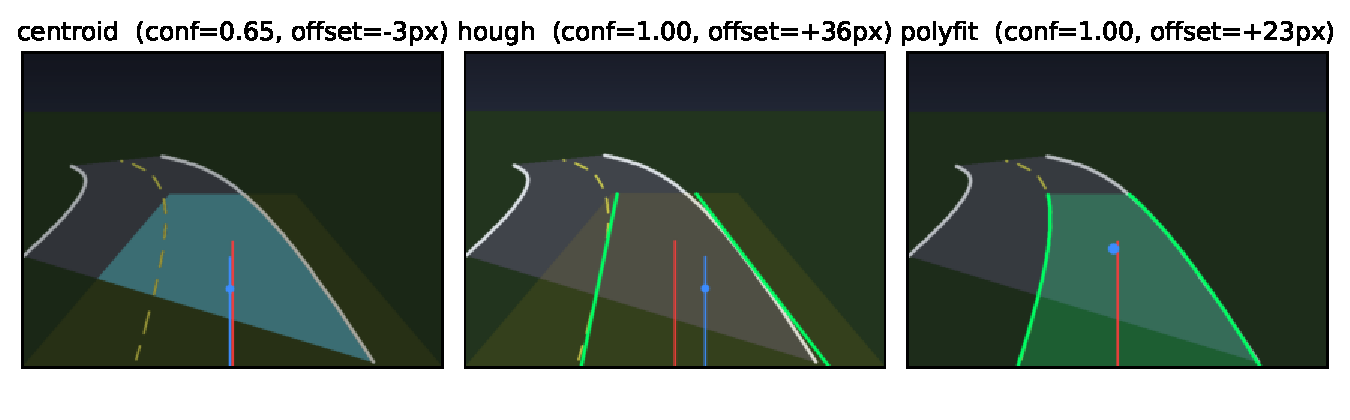
\includegraphics[width=\linewidth]{figures/annotations.pdf}
  \caption{Same camera frame, three detectors. Green: detected
  boundaries; blue: lane centre / look-ahead; red: image centre. The
  Hough detector (centre) fits straight lines that chord the curve;
  the polynomial-fit detector (right) traces the bend.}
  \label{fig:annot1}
\end{figure}

\subsection{Why the Hough detector misses curves}

The Hough detector's model class is the set of straight lines. On a
curve, however, the actual lane boundary is not in this class -- the
best the detector can do is return the straight line that ``best
fits'' the visible curved edge pixels. What does ``best fit'' mean
under the length-weighted average from \eqref{eq:lwavg}?

Geometrically, the averaged line is biased toward the \emph{chord} of
the curve within the ROI. Consider a right-bending lane: the visible
left boundary in the ROI starts at, say, $(80, 480)$ at the bottom and
exits at $(280, 216)$ at the ROI top. The edge pixels lie on a curve
that bows away from the chord -- but a straight-line fit can only
report the chord. The lane centre (midpoint of the two chords)
therefore underestimates how far right the road actually goes at the
look-ahead row.

This bias is small on shallow bends and grows quickly on tight ones.
Worse, because the model is wrong everywhere on the curve, the
detector cannot look ahead: the line drawn at the top of the ROI is
just the same straight line extrapolated, not a faithful prediction of
where the road will be. The controller therefore has no warning of an
upcoming sharp bend until the bend has already started filling the
bottom of the image.

Experimentally (see Table in the report,
\texttt{presentation/figures/summary\_table.tex}) the Hough detector
manages to complete every track in this study, but its RMS lateral
error is $25.4$\,px on average -- nearly an entire lane-width
oscillation amplitude on the narrower circuits. Its mean lane-IoU is
only $0.24$, compared to $0.33$ for the polyfit detector. The
proposed remedy -- model the lane as a polynomial in a top-down view
rather than a line in the perspective view -- is the subject of the
second half of this document.
